\section{Durchführung und Aufbau}
\label{sec:Durchführung}
\subsection{Versuchsaufbau}
Zentrales Element des Versuchaufbaus ist ein Peltier Element womit vier verschiedene Metalle gekühlt bzw erwärmt werden. Die Temperatur der Stäbe wird an jeweils 2 verschieden Punkten gemessen und auf einem Messgerät ausgegeben. Die beiden Thermoelemente liegen jeweils 3 \si{\cm} auseinander. Mittels GLX können die Temperaturverläufe dargestellt und Differenzen berechnet werden.

\begin{figure}[ht]
	\centering
	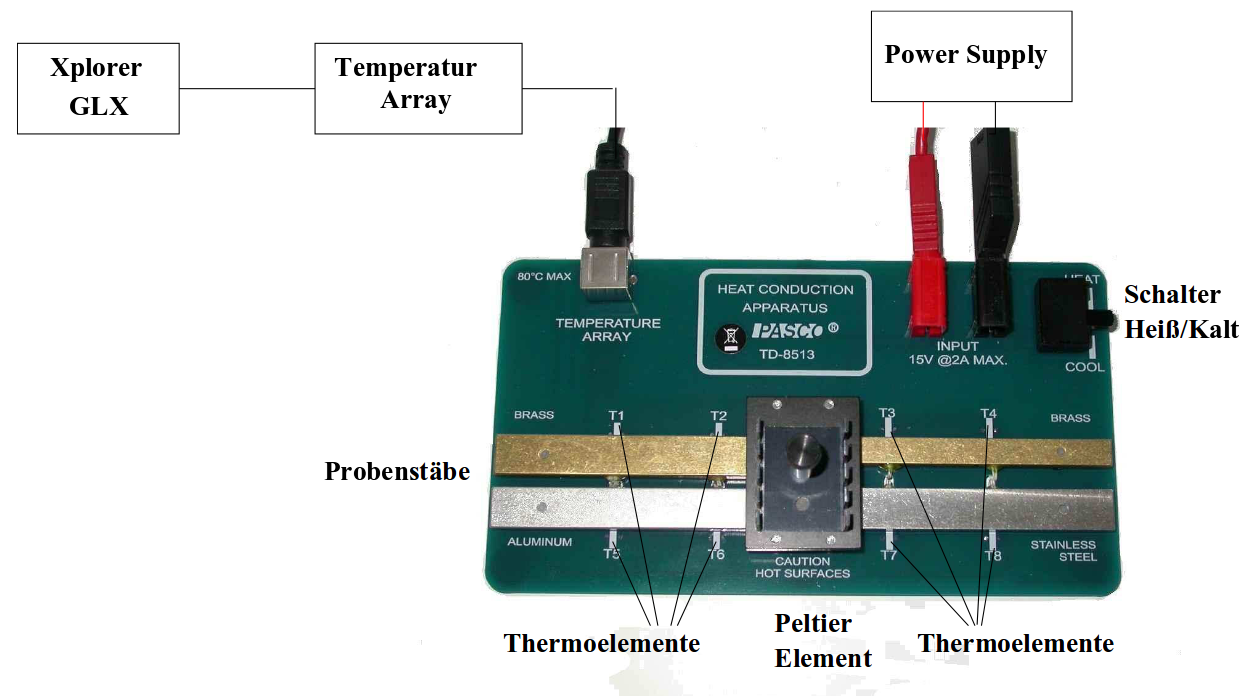
\includegraphics[height=5cm]{./Aufbau.png}
	\caption{Experimenteller Aufbau zur Bestimmung der Wärmeleitfähigkeit \cite{Aufbau}.}
	\label{fig:Aufbau}
\end{figure}



\subsection{Peltier Element}
Die Funktionsweise eines Peltier Elements beruht auf dem Seebeck-Effekt bzw. Peltiereffekt. Grundlage dessen sind zwei miteinander verbundene Halbleiter mit unterschiedlichen Energieniveaus. Bei einem Stromfluss durch die Metalle kommt es durch den Kontakt zu einem Potentialausgleich. Wenn die Elektronen durch den Stromfluss in ein energetisch günstigeren Zustand übergehen wird Wärme frei, falls sie in einen höherenergetischen Zustand gelangen wird der Umgebung Wärme entzogen um die Potentialdifferenz zu überbrücken.


\subsection{Statische Methode}
Hierbei werden die vier Stäbe durch das Peltier Element solange geheizt bis das siebte Thermoelement (siehe Abbildung \ref{fig:Aufbau}) eine Temperatur von $45^\circ$ Celsius misst. Das Peltier Element wird mit einer Eingangsspannung von 7 Volt betrieben bei maximaler Stromstärke. Die Temperatur der einzelnen Thermomelemente wird jede fünf Sekunden mittels des GLX Xplorers ausgelesen. Auf diesem werden die Temperaturverläufe T1 und T4 sowie T5 und T8 graphisch gegeinander aufgetragen. Zusätzlich wird eine Temperaturmessung nach 700 Sekunden an dem ersten, vierten, fünften und achten Thermoelement durchgeführt um die beste Wärmeleitung der Stäbe zu bestimmen. Außerdem sollen die Temperaturdifferenzen T2-T1 und T7-T8 graphisch dargestellt werden.

\subsection{Dynamische Methode}
Mittels des Angström-Messverfahren wird der Stab nun periodisch geheizt, so dass eine Temperaturwelle entsteht. Durch die Phasengeschwindigkeit der Welle lässt sich die Wärmeleitfähigkeit bestimmen. \ \\
Bei dem Versuchsaufbau wird eine Abtastrate der Temperatur von zwei Sekunden und eine Periodendauer von 80 Sekunden der Heiz- bzw. Kühlphase eingestellt. Das Peltier Element wird mit einer Eingangsspannung von 10 Volt bei maximaler Stromstärke betrieben. Die Messung wird über 10 Perioden betrieben und anschließend der Temperaturverlauf für den breiten Messingstab (T1 und T2) graphisch dargestellt.
Im Anschluss kühlen die Stäbe auf minimal $30^\circ$ Celsius herunter und der Versuch wird analog mit einer Periodendauer von 200 Sekunden durchgeführt. Dieses mal wird der temperaturverlauf an den Thermoelementen T7 und T8 welche an einem Edelstahlstab befestigt sind graphisch dargestellt.
